\documentclass{article}
\usepackage[utf8]{inputenc}
\usepackage{amsmath, amssymb, tikz, graphicx}
\usepackage{enumitem}
\usepackage{graphicx}
\usepackage[margin=1in]{geometry} % Paquete geometry para ajustar márgenes
\usepackage{float}

\title{Cálculo Integral I-2025 301-302}
\author{Johan Sebastián Posada Beltrán}
\date{\today}

\begin{document}

\maketitle


\section{Actividad I Introducción}

Fecha de Entrega: Aula Virtual.

A continuación, encontrará una serie de actividades que sirven para reforzar, analizar y evaluar los aprendizajes mínimos para iniciar el curso de Cálculo Integral. Esta actividad se debe subir en formato pdf generado por un editor de textos científicos.
\section{Repaso}

La intención de las siguientes preguntas es repasar y recordar algunos conceptos básicos que debe tener en cuenta para desarrollar esta tarea e iniciar el curso de cálculo integral.

\begin{itemize}
    \item \textit{Pregunta 1} ¿Qué es una función real, el dominio, el rango y la gráfica de una función real?
    \item \textit{Pregunta 2} ¿Cuál es la definición de valor absoluto?
    \item \textit{Pregunta 3} ¿Qué relación existe entre el concepto de límite de una sucesión o una función con el concepto de valor absoluto?
    \item \textit{Pregunta 4} ¿Qué significa que exista y calcular, el límite de una función real en un punto de su dominio?
    \item \textit{Pregunta 5} ¿Qué es la derivada de una función real en un punto de su dominio? Explique en sus palabras el significado de tasa de cambio instantáneo, qué es la recta tangente a la gráfica de una función en un punto de su dominio, si todas las funciones reales son diferenciables y si el concepto de derivada es global o local en el dominio.
    \item \textit{Pregunta 6} ¿Cuál es la relación entre el concepto de límite y el de derivada?
\end{itemize}
\section{Problemas Rutinarios}

Se espera que las siguientes actividades le permitan comprender, repasar y utilizar propiedades y métodos analíticos que aprendió en el curso de Cálculo Diferencial:

\begin{enumerate}
    \item Determine la ecuación de la recta tangente a la función \(f(x)=x^2+3x-5\) en \(x=1\).
    \item Encuentre los puntos críticos y clasifíquelos como máximos, mínimos o puntos de silla para la función \(f(x)=x^3-6x^2+9x+2\).
    \item Analice la continuidad de la función:
    $$
    f(x)=\begin{cases}
    x^2-1, & x<2, \\
    3x-5, & x\geq 2.
    \end{cases}
    $$
    \item Use herramientas de cálculo para hacer un \emph{sketch} de la gráfica de las siguientes funciones, además, describa el paso a paso para llegar a su \emph{sketch}:
    \begin{enumerate}
        \item \(f(x)=\frac{x}{x^2-1}\),
        \item \(f(x)=\frac{1}{(x-1)(x-3)}\),
        \item \(f(x)=x+\frac{1}{x^2}\).
    \end{enumerate}
\end{enumerate}
\section{Geometría Cartesiana}
En las secciones 1.1, 1.2 y 1.3 del libro \cite{4} se encuentran los conceptos básicos sobre plano Cartesiano y funciones:

\section*{Ideas básicas}
\begin{itemize}
    \item La geometría cartesiana es fundamental para el desarrollo del cálculo integral, ya que permite representar puntos en el plano mediante coordenadas numéricas.
    \item El plano Cartesiano es un sistema de referencia, es decir, permite ubicar puntos mediante coordenadas, fue introducido por René Descartes (1596-1650) y se basa en el uso de un sistema de ejes perpendiculares.
\end{itemize}

Para el sistema de coordenadas cartesianas:
\begin{itemize}
    \item Se utilizan dos rectas perpendiculares: una horizontal (\textbf{eje x}) y otra vertical (\textbf{eje y}).
    \item El punto de intersección de los ejes es el \textbf{origen (O)}.
    \item Cada punto en el plano se representa mediante un par ordenado $(x,y)$, donde:
    \begin{itemize}
        \item $x$ es la \textbf{abscisa} (distancia al eje y).
        \item $y$ es la \textbf{ordenada} (distancia al eje x).
    \end{itemize}
    \item Los signos de las coordenadas determinan el cuadrante en el que se encuentra el punto:
    \begin{itemize}
        \item \textbf{Primer cuadrante}: $x > 0, y > 0$
        \item \textbf{Segundo cuadrante}: $x < 0, y > 0$
        \item \textbf{Tercer cuadrante}: $x < 0, y < 0$
        \item \textbf{Cuarto cuadrante}: $x > 0, y < 0$
    \end{itemize}
\end{itemize}

\subsubsection*{Espacio tridimensional}
\begin{itemize}
    \item En el espacio, se utilizan tres ejes perpendiculares $(x, y, z)$ que se cortan en el origen.
    \item Cada punto en el espacio se describe mediante tres coordenadas $(x, y, z)$.
\end{itemize}

\subsubsection*{Aplicaciones geométricas}
\begin{itemize}
    \item La ecuación de la circunferencia $r^2 = x^2 + y^2$, representa un punto $(x, y)$ que está a una distancia $|x|$ unidades desde el origen haste el eje vertical y una distancia $|y|$ desde el origen hasta el eje horizontal.
\end{itemize}

\subsection*{Funciones. Ideas generales y ejemplos}

De manera informal se puede decir que asigna a cada elemento $x$ de un conjunto $X$ (dominio) un único elemento $y$ de otro conjunto $Y$ (imagen).

Las funciones pueden representarse de varias maneras:
\begin{itemize}
    \item \textbf{Gráficas}: Los puntos $(x, f(x))$ forman la gráfica de la función en el plano cartesiano.
    \item \textbf{Tablas}: Muestran pares $(x, y)$ de manera explícita.
    \item \textbf{Fórmulas}: Expresan la relación entre $x$ y $y$ mediante ecuaciones algebráicas.
\end{itemize}

\subsubsection*{Ejemplos de funciones}
\begin{itemize}
    \item \textbf{Función identidad}: $f(x) = x$. Su gráfica es una recta que pasa por el origen y forma ángulos iguales con los ejes.
    \item \textbf{Función número primo}: $\pi(x)$, que cuenta los números primos menores o iguales a $x$. Su gráfica consiste en segmentos horizontales con saltos en los números primos.
    \item \textbf{Función factorial}: $f(n) = n!$, que calcula el producto de todos los enteros positivos hasta $n$.
    \item \textbf{Función valor absoluto}: $\phi(x) = |x|$. Asigna a cada número real $x$ su valor absoluto.
\end{itemize}

\subsubsection*{Propiedades del valor absoluto}

\begin{multicols}{2}
\begin{enumerate}[label=(\arabic*)]
    \item
    \[
        |x| = \sqrt{x^2}
    \]

    \item
    \[
        |x|^2 = x^2
    \]

    \item
    \[
        x + b \leq |x + b|
    \]

    \item
    \[
        |x - b| = |b - x|
    \]

    \item
    \[
        |x| \geq 0
    \]

    \item
    \[
        |xy| = |x|\cdot|y|
    \]

    \item
    \[
        \left|\frac{x}{y}\right| = \frac{|x|}{|y|} 
        \quad (\text{con } y \neq 0)
    \]

    \item
    \[
        |x + y| \leq |x| + |y|
    \]

    \item
    \[
        ||x| - |y|| \leq |x - y|
    \]

    \item
    \[
        |x| < a 
        \;\;\Leftrightarrow\;\; -a < x < a 
        \quad (\text{para } a > 0)
    \]

    \item
    \[
        |x| \leq a 
        \;\;\Leftrightarrow\;\; -a \leq x \leq a 
        \quad (\text{para } a > 0)
    \]

    \item
    \[
        |x| > a 
        \;\;\Leftrightarrow\;\; x < -a \;\text{o}\; x > a 
        \quad (\text{para } a > 0)
    \]

    \item
    \[
        |x| \geq a 
        \;\;\Leftrightarrow\;\; x \leq -a \;\text{o}\; x \geq a 
        \quad (\text{para } a > 0)
    \]
\end{enumerate}
\end{multicols}

\subsubsection*{Propiedades de las funciones}
\begin{itemize}
    \item Para cada $x$ en el dominio $X$, existe un único $y$ en el recorrido $Y$.
    \item Dos pares $(x, y)$ y $(x, z)$ no pueden existir con el mismo $x$ y valores distintos de $y$.
\end{itemize}

\section*{Funciones. Definición formal como conjunto de pares ordenados}

Una función \( f \) es un conjunto de pares ordenados \( (x,y) \), donde:
\begin{itemize}
    \item Cada \( x \) en el dominio \( X \) tiene exactamente un \( y \) asociado.
    \item Dos pares \( (x,y) \) y \( (x,z) \) no pueden existir con el mismo \( x \) y valores distintos de \( y \).
    \item La imagen de  \( x \) se denota como \( f(x) \).
\end{itemize}

\subsubsection*{Dominio y recorrido}
\begin{itemize}
    \item El \textbf{dominio} de \( f \) es el conjunto de todos los \( x \) que aparecen como primeros elementos en los pares \( (x,y) \).
    \item El \textbf{recorrido} de \( f \) es el conjunto de todos los \( y \) que aparecen como segundos elementos en los pares \( (x,y) \).
\end{itemize}

\subsubsection*{Representación de funciones}
\begin{itemize}
    \item Una función puede imaginarse como una tabla con dos columnas: una para los valores de \( x \) (dominio) y otra para los valores de \( y \) (recorrido).
    \item Para todo \( x \) en el dominio de \( f \), existe exactamente un \( y \) tal que \( (x,y) \in f \).
\end{itemize}

\subsubsection*{Teorema sobre la igualdad de funciones}
\begin{itemize}
    \item Tienen el mismo dominio.
    \item \( f(x) = g(x) \) para todo \( x \) en el dominio.
\end{itemize}

\section{Problemas No Rutinarios}

Si \(f\) es una función continua en un intervalo cerrado \([a, b]\), excepto quizás en un punto \(c\in[a,b]\), determine la veracidad o falsedad de los siguientes enunciados (justifique su respuesta):

\begin{itemize}
    \item Si \(f'(x)\) es positiva para todo \(x<c\), y \(f'(x)\) es negativa para todo \(x>c\), en el punto \(c\) hay un máximo relativo de \(f\).
\end{itemize}

El enunciado en pocas palabras establece que si que a la izquierda de $c$ la función es creciente  ($f'(x) > 0$ para $x < c$) y a la derecha de $c$ es decreciente  ($f'(x) < 0$ para $x > c$) , entonces hay un máximo relativo. Esto no es cierto porque la función debe ser continua en todo el intervalo $[a, b]$, si $c \in [a, b]$ entonces la función no tiene un punto crítico. El criterio de la primera derivada dice que para analizar el crecimiento de una función es necesario calcular en qué casos dicha derivada vale cero o no existe.

Hay que tener en cuenta de que si una función crece a la izquierda y decrece a la derecha de $c$ o viceversa, no significa siempre que exista un máximo o un mínimo relativo en $[a, b]$ de $f$, pues puede darse el caso de que en $c$ existan asíntotas como se aprecia en la función racional de la figura \ref{fig:racional1}. Un punto crítico es donde la derivada de la función es cero, sin embargo puede existir un punto de discontinuidad, allí la derivada no existe, pero puede crecer o decrecer sin necesidad de ser un máximo o un mínimo.

En cambio, en la función cuadrática de la figura \ref{fig:cuadratica1} no hay una asíntota y aparentemente es un máximo, pero no lo es porque allí la derivada no existe. \textbf{Por lo tanto el enunciado es falso}.

\begin{figure}[H]
    \centering
    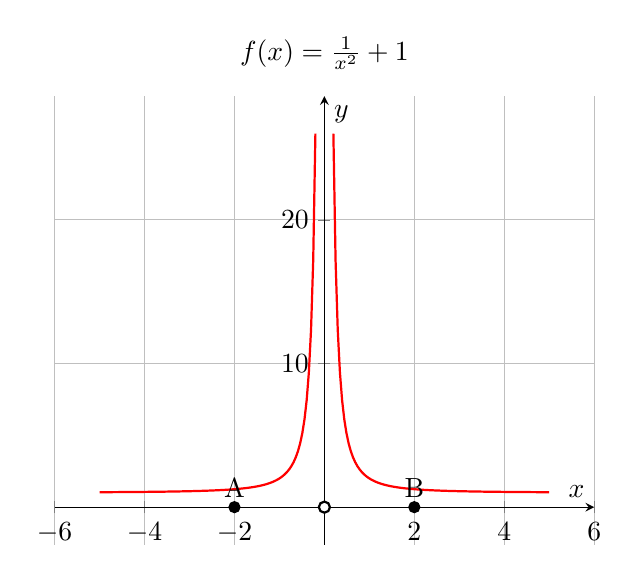
\begin{tikzpicture}
    \begin{axis}[
        title={$f(x) = \frac{1}{x^2} + 1$},
        axis lines = middle,
        grid = major,
        enlargelimits = true,
        xlabel={$x$},
        ylabel={$y$},
    ]
    
    % Función racional
    \addplot[domain=-5:-0.2, samples=100, thick, red] {((1)/(x^(2)))+1};
    \addplot[domain=0.2:5, samples=100, thick, red] {((1)/(x^(2)))+1};
    
    % Puntos marcados
    \addplot[only marks, mark=*, mark options={black}, nodes near coords={A}] coordinates {(-2,0)};
    \addplot[only marks, mark=*, mark options={black}, nodes near coords={B}] coordinates {(2,0)};
    \addplot[only marks, mark=*, mark options={white}, scale=1.5] coordinates {(0,0)};
    \addplot[only marks, mark=o, mark options={black}, scale=1.5, thick] coordinates {(0,0)};
    
    \end{axis}
\end{tikzpicture}
    \caption{Función racional decreciente y creciente antes y después de $c$ respectivamente.}
    \label{fig:racional1}
\end{figure}

\begin{figure}[H]
    \centering
    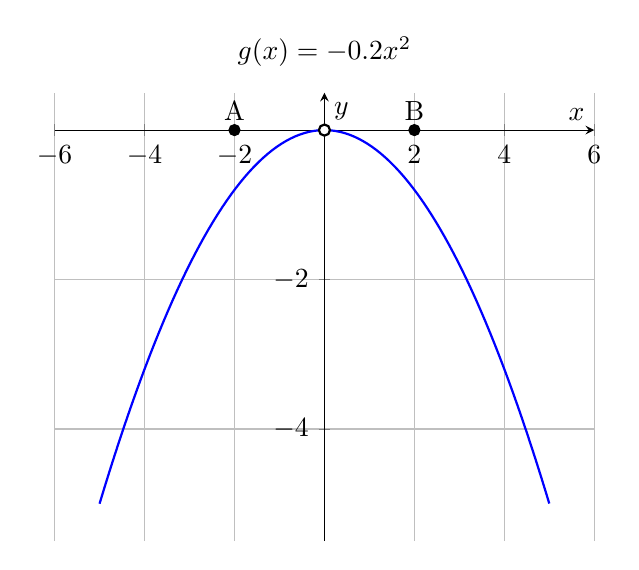
\begin{tikzpicture}
    \begin{axis}[
        title={$g(x) = -0.2x^2$},
        axis lines = middle,
        grid = major,
        enlargelimits = true,
        xlabel={$x$},
        ylabel={$y$},
    ]
    
    % Función cuadrática
    \addplot[domain=-5:5, samples=100, thick, blue] {-0.2*x^2};
    
    % Puntos marcados
    \addplot[only marks, mark=*, mark options={black}, nodes near coords={A}] coordinates {(-2,0)};
    \addplot[only marks, mark=*, mark options={black}, nodes near coords={B}] coordinates {(2,0)};
    \addplot[only marks, mark=*, mark options={white}, scale=1.5] coordinates {(0,0)};
    \addplot[only marks, mark=o, mark options={black}, scale=1.5, thick] coordinates {(0,0)};
    
    \end{axis}
\end{tikzpicture}
    \caption{Función cuadrática decreciente y creciente antes y después de $c$ respectivamente.}
    \label{fig:cuadratica1}
\end{figure}

\begin{itemize}
    \item Si \(f'(x)\) es negativa para todo \(x<c\), y \(f'(x)\) es positiva para todo \(x>c\), en el punto \(c\) hay un mínimo relativo de \(f\).
\end{itemize}

En este enunciado se podría aplicar la misma lógica que en el primero, pero abordaré en este el criterio de la segunda derivada. Una vez se hallan los puntos críticos igualando la primera derivada a cero, entonces se evavlúa la segunda derivada en dichos puntos y si $f''(x) > 0$ entonces la función es cóncava hacia arriba y si $f''(x) < 0$ entonces la función es cóncava hacia abajo.

Si la función es cóncava hacia arriba en un punto crítico, entonces es un mínimo relativo y si es cóncava hacia abajo, entonces es un máximo relativo. Sin embargo, en este caso no existen puntos críticos, ya que al igualar $f'(x) = 0$ no se obtiene ninguna solución. \textbf{Por lo tanto, el enunciado es falso}.

En las siguientes gráficas se puede apreciar lo anteriormente mencionado:

\begin{figure}[H]
    \centering
    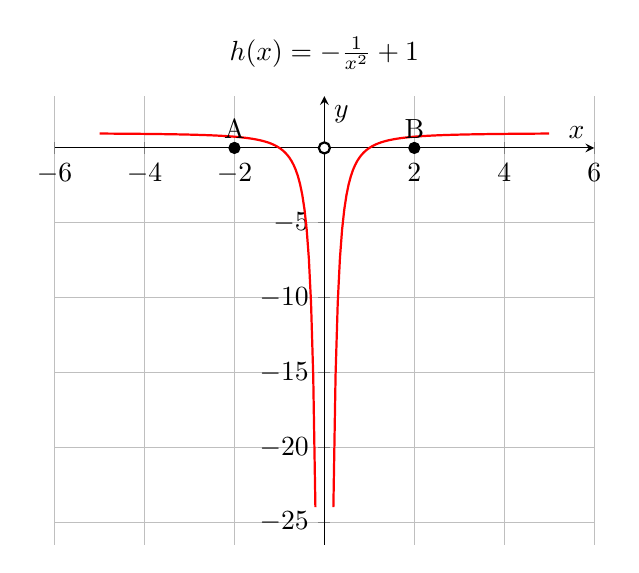
\begin{tikzpicture}
    \begin{axis}[
        axis lines = middle,
        grid = major,
        enlargelimits = true,
        xlabel={$x$},
        ylabel={$y$},
        title={$h(x) = -\frac{1}{x^2} + 1$}
    ]
    
    % Función racional
    \addplot[domain=-5:-0.2, samples=100, thick, red] {-((1)/(x^(2)))+1};
    \addplot[domain=0.2:5, samples=100, thick, red] {-((1)/(x^(2)))+1};
    
    % Puntos marcados
    \addplot[only marks, mark=*, mark options={black}, nodes near coords={A}] coordinates {(-2,0)};
    \addplot[only marks, mark=*, mark options={black}, nodes near coords={B}] coordinates {(2,0)};
    \addplot[only marks, mark=*, mark options={white}, scale=1.5] coordinates {(0,0)};
    \addplot[only marks, mark=o, mark options={black}, scale=1.5, thick] coordinates {(0,0)};
    
    \end{axis}
\end{tikzpicture}
    \caption{Función racional creciente y decreciente antes y después de $c$ respectivamente.}
    \label{fig:racional2}
\end{figure}

\begin{figure}[H]
    \centering
    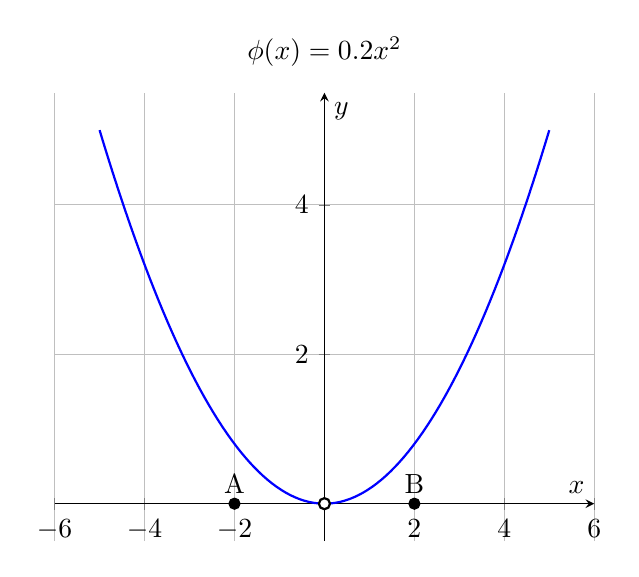
\begin{tikzpicture}
    \begin{axis}[
        title={$\phi(x) = 0.2x^2$},
        axis lines = middle,
        grid = major,
        enlargelimits = true,
        xlabel={$x$},
        ylabel={$y$},
    ]
    
    % Función cuadrática
    \addplot[domain=-5:5, samples=100, thick, blue] {0.2*x^2};
    
    % Puntos marcados
    \addplot[only marks, mark=*, mark options={black}, nodes near coords={A}] coordinates {(-2,0)};
    \addplot[only marks, mark=*, mark options={black}, nodes near coords={B}] coordinates {(2,0)};
    \addplot[only marks, mark=*, mark options={white}, scale=1.5] coordinates {(0,0)};
    \addplot[only marks, mark=o, mark options={black}, scale=1.5, thick] coordinates {(0,0)};
    
    \end{axis}
\end{tikzpicture}
    \caption{Función cuadrática creciente y decreciente antes y después de $c$ respectivamente.}
    \label{fig:cuadratica2}
\end{figure}
\section{Análisis Numérico o Computacional}

\begin{enumerate}
    \item Use el método de la bisección para encontrar una aproximación a la raíz de la ecuación \(f(x)=x^3-x-2\) en el intervalo \([1,2]\) con una tolerancia de \(10^{-3}\).
    \item Aproxime la derivada de \(f(x)=e^x\) en \(x=1\) usando diferencias finitas progresivas con \(h=0.1\).
\end{enumerate}

\begin{thebibliography}{9}
    \bibitem{1} Stewart J. -- \emph{Calculus Concepts and Contexts}, 2ª ed., Thomson (2004).
    \bibitem{2} Boyce, W. E.; DiPrima, R. C.; Meade, D. B. -- \emph{Elementary Differential Equations and Boundary Value Problems}, Wiley (2021).
    \bibitem{3} Marsden, J.; Tromba, A. -- \emph{Cálculo Vectorial}, (1991).
    \bibitem{4} Apostol, T. -- \emph{Calculus Volumen I: Cálculo con funciones de una variable, con una introducción al álgebra lineal}, 2ª ed., Reverte (2001).
\end{thebibliography}

\end{document}